\documentclass[12pt,UTF8,fntef]{article}
\usepackage[left=1.8cm, right=1.8cm, top=1.8cm, bottom=1.8cm]{geometry}
%\usepackage[utf8]{inputenc}
\usepackage[english]{babel}
\usepackage{graphicx}
\usepackage[unicode, pdfborder={0 0 0}, bookmarksdepth=-1]{hyperref}
\usepackage[usenames, dvipsnames]{color}
\usepackage[shortlabels, inline]{enumitem}
\usepackage{fancyhdr}
\usepackage{amssymb}
\usepackage{amsmath}
\usepackage{hyperref}
\usepackage{subfigure}
\usepackage{float}
\usepackage{spreadtab}
\usepackage{cite}
\usepackage{siunitx}
\usepackage{enumitem}
\usepackage{tikz}
\usepackage{pgfplotstable}

\pgfplotsset{width=15cm}
\pgfplotsset{height=8cm}
\pgfplotsset{compat=1.16}

\hypersetup{
    pdftoolbar=true,        % show Acrobat’s toolbar?
    pdfmenubar=true,        % show Acrobat’s menu?
    pdffitwindow=false,     % window fit to page when opened
    pdfstartview={FitH},    % fits the width of the page to the window
    %pdftitle={前瞻語音計畫申請},    % title
    pdfauthor={Jui-Yang Hsu},     % author
    pdfnewwindow=true,      % links in new PDF window
    colorlinks=true,       % false: boxed links; true: colored links
    linkcolor=purple,          % color of internal links (change box color with linkbordercolor)
    citecolor=blue,        % color of links to bibliography
    filecolor=magenta,      % color of file links
    urlcolor=cyan           % color of external links
}

%\usepackage[square,numbers]{natbib}
%\bibliographystyle{abbrvnat}
\renewcommand{\baselinestretch}{1.25}
\usepackage{xeCJK}
\usepackage{fontspec}
%\setCJKmainfont{DFFN_R3.TTC}
\setCJKmainfont[BoldFont=Noto Serif CJK TC Bold]{Noto Serif CJK TC}
\title{研究計畫書}
\author{電機工程研究所~~~計算機科學組\\R07921053~~~徐瑞陽 \\ 技術部落格: \texttt{https://sunprinces.github.io/learning/}}
%\email{r07921053@ntu.edu.tw}
\date{}

\begin{document}

\maketitle

\begin{section}{學生背景}
  \begin{subsection}{語音技術相關課程修習}
~~~~學生徐瑞陽畢業於臺大電機系,在大二時修習了李宏毅老師所開設的機器學習及其深層與結構化之課程,初探了深度學習的技術,並於大三開始在語音實驗室進行專題研究。在大三為期一年的專題中,與同學方為一起進行了機器智慧問答系統的研究,利用樹型長短期記憶網路 (Tree-structured Long Short-Term Memory, TreeLSTM) 與記憶網路 (Memory Network) ,端對端地訓練機器根據所問的問題,從文本當中擷取相關資訊並做出回答,在托福聽力測驗這個語料庫上,達到了當時最好的結果,並於 2016 年的 SLT 國際會議發表成果。

    除了在專題研究中累積的文獻閱讀與實做經驗,學生也修習了數位語音處理、機器學習、數據分析學、語言分析、基因遺傳演算法、神經資訊學等相關課程,並參與了強化學習的讀書會,充實自己在語音、自然語言及機器學習各個面向的相關知識。
  \end{subsection}

  \begin{subsection}{實習及相關經驗}
    ~~~~學生於大五時至瑞典的皇家理工學院 (KTH) 交換一年,與來自歐陸各國的學生們互相交流切磋。並於交換期結束後,至蘋果公司總部的自然語言團隊擔任實習生,為期三個月的實習期,讓自己的能力提升到另一個檔次,而與團隊中另一位實習生方為所參與的專案,也已於今年的 WWDC 亮相,將會在今年 9 月出現在 iOS 13 中。

    %於碩一時,學生擔任語音實驗室之網管,管理叢集運算資源,深入了解並維護前任網管所引進的 Slrum 工作排程系統,讓同學們在跑實驗時,能不必擔心彼此搶佔同一資源致使雙方程式均無法運行的問題,並以 Go 語言整合 netdata,改寫原先不穩定的資源監控後端。同時也增添了更多新節點部署的自動化腳本、節點損壞的自動移除與通報機制及設計更好的資源分配策略,讓實驗室同學在使用上更為便利,也讓網管的工作能更順利地交接給下一屆同學。
    於碩一時,學生擔任語音實驗室之網管,管理叢集運算資源,深入了解並維護前任網管所引進的 Slrum 工作排程系統,讓同學們在跑實驗時,不必擔心彼此搶佔同一資源致使雙方程式均無法運行的問題,並以 Go 語言整合 netdata,改寫原先不穩定的資源監控後端。同時也增添了節點損壞的自動檢查與通報機制,及設計更好的資源分配策略,讓實驗室同學在使用上更為便利,也讓網管的工作能更順利地交接給下一屆同學。
  \end{subsection}
\end{section}

\begin{section}{研究主題: Language Adaptative Training in End-to-end Speech Recognition using Meta Learning}
~~~~近年來深度學習技術已經應用於許多語音的相關領域,並取得突破性的成果,如聲音轉換、智慧問答系統、語音辨識...等。在語音辨識的研究中,利用神經網路與隱式馬可夫模型的混合模型 (DNN-HMM Hybrid Model) 建構以音素 (phoneme) 為單位的聲學模型,再利用發音字典 (lexicon) 與遞歸神經網路 (Recurrent Neural Network) 所訓練的語言模型來做語音辨識為目前最常被使用的架構。然而,這樣的架構除了要有每段語音 (utterance) 對應的翻譯之外,亦需事先用字典及維特比演算法 (Viterbi Algorithm) 對音素及幀 (frame) 做初步對齊後才能進行訓練,因為標註字典的成本昂貴且門檻較高,這樣的設定對於多數的非主流研究語言是不切實際的。

因此,Graves 等人提出了端對端的語音辨識系統之構想\cite{graves2014towards},近年來也有許多相關模型被提出,如百度的 DeepSpeech \cite{hannun2014deep}、Google 的 LAS \cite{chan2016listen} (架構如 Figure \ref{fig:monoASR} 所示)...等。這些模型主要以序列到序列模型 (Sequence-to-Sequence Model) 作為核心,配合利用專注機制 (Attention) 的解碼器與以 Connectionist Temporal Classification (CTC) 為目標函數的解碼器,訓練出輸入為音訊,輸出為字位 (grapheme) 的端對端模型,同時整合了聲學模型與語言模型的訓練,並移除了需要字典的前提。

  然而,相關文獻中均提到了端對端模型相較 DNN-HMM ,若要達到相同詞錯誤率 (Word Error Rate, WER)的情況下,需要更多訓練資料,對於語料量本來就不足的非主流語言來說,這樣的前提也使得該架構難以應用於實務中。也因此,如何利用多語料語言 (high-resource language) 去輔助訓練少語料語言(low-resource language) 的方法 - 語言自適應訓練 (Language Adaptative Training, LAT) 為近年來語音界的主要研究方向之一,在本章中,我會先介紹我所選擇的方法 - 元學習 (Meta Learning),及其在其他領域的應用,再介紹目前 LAT 的主流方法 - 遷移學習 (Transfer Learning) ,及為什麼元學習比其更適合實做 LAT,以及相較於其他應用,將元學習應用在語音領域有何不同之處,及這樣的不同會帶來什麼樣的使用限制,最後會展示目前初步的實驗結果。



  \begin{subsection}{元學習介紹}
~~~~目前在監督式學習 (Supervised Learning) - 給定特定任務的大型資料集,從頭開始訓練模型的情境下,深度學習已經取得了很大的成功。然而,相較於人類在學習新任務時,給定少量樣本便能完成學習的情況,其對資料的利用顯然是沒有效率的。而人類之所以能快速學習,主因是我們有元學習 (Meta Learning),又稱為學習如何學習 (Learning to Learn) 的能力,能從先前的任務學習過程中,發現可借鑒的通用經驗,利用已習得的技能,達到快速學習新技能的目的。以下會定義元學習,並介紹及分類近年來提出的方法。

    \begin{subsubsection}{定義}
      ~~~~以下定義 $\theta$ 為想優化的模型參數,$\mathcal{D}$ 為資料集,$\mathcal{A}$ 為衡量參數在資料集上好度的函數 (如分類問題中的最大似然),元學習的目標為

      \begin{equation}
        \theta^{\star} = \arg \max_\theta \mathbb{E}_{\mathcal{D} \sim p(\mathcal{D}) }[\mathcal{A}_\theta(\mathcal{D})]
      \end{equation}

      也就是,我們希望能找到一組參數,在不同的資料分佈中,平均而言有最好的結果\footnote{元學習是以資料集為單位,而監督式學習是以樣本為單位}。

      為了更好的理解元學習,我們來看一個其最常被使用的情境 - 少量樣本分類 (Few-shot Classification)。在這樣的情境下,對每個任務 (task) 我們都只有少量的訓練資料,但有多個任務可以學習。舉例來說,我們擁有數個二元分類的資料集 (狗 vs 貓, 火車 vs 飛機, 蘋果 vs 香蕉...),但每個資料集的每個類別都只有 $N$ 個訓練樣本 ($N \geq 1$),給定一個新資料集 (鳥 vs 船,且此類別都沒有出現在先前的資料集中),我們希望訓練出的模型能做到僅利用 $2N$ 張樣本便自適應 (adapt) 到新資料集上。

      %在這樣的情境下,對於每個特定任務我們都只有少量的訓練資料,但有多個任務可以學習,目標為

      %\begin{equation}
   %\theta^\star = \arg \max_\theta \mathbb{E}_{L \subset \mathcal{L}} \, [ \mathbb{E}_{S^L \subset \mathcal{D}, B^L \subset \mathcal{D}}[\sum_{(x,y) \in B^L} \log P_\theta(y|x,S^L)] \,  ]
       %\end{equation}
    \end{subsubsection}

    \begin{subsubsection}{基於度量的元學習方法 (Metric-based Approach)}
  主體在學習一個好的特徵編碼器 (feature encoder),而經過該編碼器編碼後的特徵,再餵給核函數 (kernel function) 判斷樣本的相似程度 (如隱空間的歐式距離或餘弦距離),進而達到分類的目的,如原型網路 (Prototypical Network) \cite{snell2017prototypical}、配對網路 (Matching Network)\cite{vinyals2016matching}...等, 此方法目前僅用於分類問題。
    \end{subsubsection}

    \begin{subsubsection}{基於模型設計的元學習方法 (Model-based Approach)}
      主體在藉由設計類似智慧問答系統的模型架構及讀寫策略,使其能利用新資料集的訓練資料來預測測試資料。如記憶增強網路 (Memory Augmented Network) \cite{santoro2016meta}利用神經圖靈機,建構一個可讀寫的外部記憶,用來儲存訓練樣本以便預測時查找。因其讀寫外部記憶的複雜度為 $\mathcal{O}(|\mathcal{D}|)$,目前僅在少量樣本分類中使用。
    \end{subsubsection}

    \begin{subsubsection}{基於優化的元學習方法 (Optimization-based Approach)} \label{opt-meta}
主體在學習訓練過程中的各個模塊如優化器\cite{ravi2016optimization}、初始參數\cite{nichol2018first, finn2017model,flennerhag2018transferring} ,或者強化學習中的損失函數、回報 (return) 的超參數...等。需注意的是,利用這組參數直接在新資料集上進行預測並不能得到理想的結果,而是以這組參數進行訓練所得的模型進行預測能有好的表現。
    \end{subsubsection}
  \end{subsection}
  \newpage

  \begin{subsection}{遷移學習應用於 LAT} \label{trans-asr}

  \begin{figure}[ht]
      \centering
      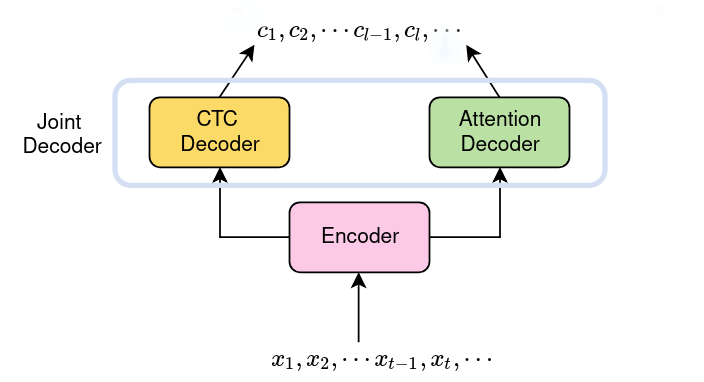
\includegraphics[width=0.6\linewidth]{monoASR.png}
      \caption{Basic learner structure: LAS}
      \label{fig:monoASR}
  \end{figure}

  \vspace{-0.25in}

  \begin{figure}[ht]
    \centering
    \subfigure[Universal ASR: Union the output classes]{%
      \label{fig:universalASR}%
    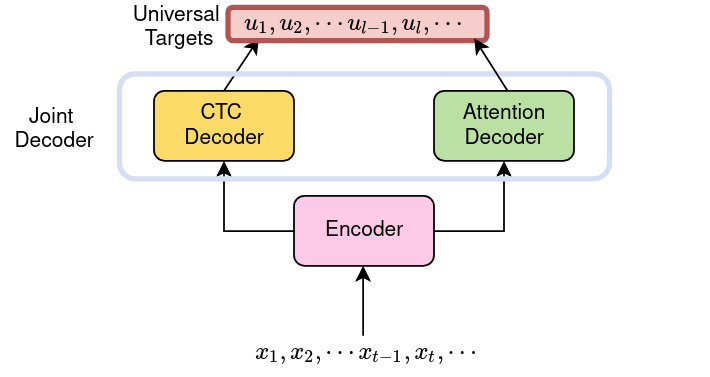
\includegraphics[width=0.55\linewidth]{UniversalASR.png}}%
    \subfigure[MultiTask ASR: Language-specific decoder]{%
      \label{fig:multitaskASR}%
    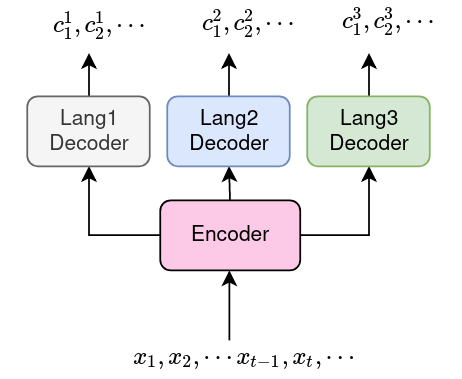
\includegraphics[width=0.41\linewidth]{MultiTaskASR.png}}%
    \caption{Baseline model: Universal ASR \& MultiTask ASR}
  \end{figure}

  目前端對端語音辨識模型 LAT 的主流方法為遷移學習。其中 Figure \ref{fig:monoASR} 為基本的模型架構,可以訓練單一語言的模型。Figure \ref{fig:universalASR} 則延伸原先的架構,統一所有訓練語料的輸出類別,可藉由聯集訓練語言的字位或使用語言通用的國際音標來實現;Figure \ref{fig:multitaskASR} 架構則是對不同語言建構各自的解碼器,分別輸出字位,但前面的編碼器是互相共享的。在遷移到目標語言時,我們將輸出層換成適合該語言的層,並重新訓練輸出層,或對整個模型進行微調 (fine-tuning) 以實現 LAT\footnote{此處不考慮將目標語言加入訓練,雖然這通常會讓結果更好,但我們希望訓練的模型對目標語言沒有任何假設}。

~~在編碼器端,為了消弭不同語言的差異,擷取出語言獨立 (language-independent) 的特徵供解碼器使用,常見的作法有加上語言分類器進行對抗訓練 (Adversarial Training),或加入音素、子字單位 (subword unit)的 CTC 解碼器。
  \end{subsection}

  \begin{subsection}{元學習應用於 LAT}
    \begin{subsubsection}{為何元學習於語音有研究價值}

  \begin{figure}[ht]
      \centering
      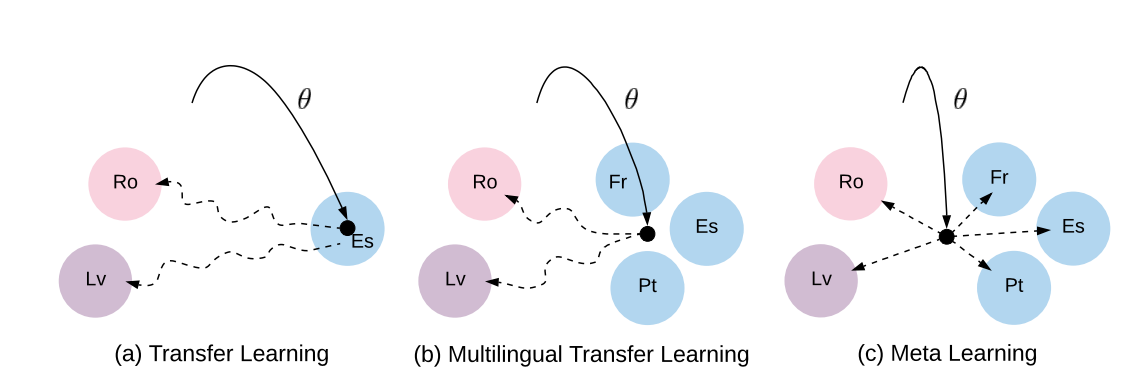
\includegraphics[width=0.8\linewidth]{Meta-motivation.png}
      \caption{不同學習之間的比較,實線為初始參數的學習過程,虛線為微調的過程}
      \label{fig:motivation}
  \end{figure}

  遷移學習以一個在多語料(多語言)訓練好的模型為基準,用於學習新的目標語言,如Figure \ref{fig:motivation} 的 (a)、(b)\footnote{圖片來自 \cite{gu2018meta}},然而問題有二︰
      \begin{enumerate}[itemsep=-1mm]
        \item 需假設訓練語料彼此的最優參數不能相差太多,因在訓練過程中必須同時滿足各語言的目標函數,這相當於對模型施加了正則化 (regularization),使其無法很好處理語種差異過大,導致正則化強度太大,無法達到最佳表現的情況。
        \item 需假設訓練語料與測試語料的最優參數不能相差太多,否則在損失平面 (loss surface) 上過長的移動,會降低找到好解的可能。 
      \end{enumerate}

      元學習中學習初始參數的方法(\ref{opt-meta}) 很好地解決了上述問題,透由在梯度更新時,將學習過程隱性編碼進所找到的參數中,使得該參數可以快速泛化到不同語言,如 Figure \ref{fig:motivation} 的 (c)所示。
    \end{subsubsection}
    \begin{subsubsection}{使用限制及挑戰} \label{meta-problem}
      目前元學習主要應用於機器視覺的少樣本分類、與強化學習,直至去年,才有了第一篇應用於機器翻譯的研究 \cite{gu2018meta},MetaNMT,訓練多語言翻譯至英文的模型,原因為以下兩點︰
      \begin{enumerate}[itemsep=-1mm]
        \item 要訓練一個成功的機器翻譯或語音辨識系統,難度相當高,不可能僅僅使用數個樣本便達到,因此多數針對少樣本分類問題的元學習演算法不適用,僅有基於優化的演算法 (\ref{opt-meta}) 在以一階梯度近似的前提下才能應用於該情境 (如 FOMAML \cite{finn2017model}、Reptile\cite{nichol2018first})。
        \item 多數學習初始參數的元學習方法雖名為與模型無關 (Model-Agnostic) ,但在使用時仍要求模型架構必須相同 (如網路中每層的神經元數量),MetaNMT 的處理方式為先將所有語言映射到相同空間,使得輸入層一致進而達到全模型一致;但在語音辨識中,雖然不同語言的輸入同為相同維度的語音特徵,輸出卻是每個語言都不同,因此無法直接套用元學習。
      \end{enumerate}
    \end{subsubsection}
    \begin{subsubsection}{初步實驗 - 音素辨識 (Framewise Phoneme Classification)}
      在將元學習應用於端對端語音辨識之前,我先嘗試音素辨識這個較為簡單的語音任務,來驗證其可行性,如 \ref{meta-problem} 所提到的模型架構問題,我放寬了對架構的假設,在每個任務的學習中,允許輸出層以同樣的方法進行權重初始化後再開始訓練,在測試時亦可置換輸出層。除此之外,相比於少樣本分類問題,我將原先對單位任務訓練資料量的限制從少樣本 (Few-shot) 放寬到少語料 (Low-resource),將對收斂速度的要求從幾步梯度就收斂放寬至快速自適應 (rapid adaptation),如一個 epoch (約數百步梯度),以更符合各語音應用的使用情境。

      我選用 TUNDRA \cite{stan2013tundra} 這個語料庫做為評斷標準,每個語言有 $4 \sim 10$小時不等的語料,比較了 MultiTask ASR 與 Meta ASR 兩種模型預訓練於 6 種語言,與完全沒有預訓練 (no-pretrain) 的模型,在目標的兩種語言訓練 5 個 epoch 後在測試資料進行預測的表現。

    \begin{figure}[H]
    \centering
    \hspace{-5.2cm}
    \begin{tikzpicture}[trim axis left, trim axis right]

    \begin{axis}[
      width=0.6\linewidth,
      legend entries={Meta ASR (on \SI{10}{\percent} data), MultiTask ASR (on \SI{10}{\percent} data), no-pretrain (on \SI{10}{\percent} data),no-pretrain (on \SI{20}{\percent} data), no-pretrain (on \SI{50}{\percent} data)} ,
          xlabel = {Number of pretraining steps},
          xmin=0,
          xmax=210,
          grid=both,
          %legend style={at={(0.65,0.62)},anchor=south west},
          legend pos=outer north east,
          ylabel={Phoneme Classification Accuracy}]
    \addplot+[smooth]table{reptile_metaval};
    \addplot+[smooth]table{ft_metaval};
     \addplot[style=ultra thick,dashed,] coordinates {(0,0.557) (200,0.557)};
     \addplot[style=ultra thick,dashed, gray] coordinates {(0,0.589) (200,0.589)};
     \addplot[style=ultra thick,dashed, brown] coordinates {(0,0.628) (200,0.628)};
    \end{axis}
    \end{tikzpicture}
    %\caption{Pretrain on EN, FI, FR, NL, RM, RU, and evaluate on }
    \caption{TUNDRA phoneme classification experiment}
    \label{fig:tundra-exp}
  \end{figure}
  從 Figure \ref{fig:tundra-exp} 可以看出,有預訓練的模型可以用較少的目標語言訓練資料便有較好的表現;且元學習的方法 (Meta ASR) 相較 MultiTask ASR\footnote{這裡並沒有比較 Universal ASR,因預訓練語言以不同的音素集 (Arpabet、GlobalPhone、Prosodylab、IPA)標註,在訓練語料不夠多的情況下,表現不甚理想},在資料量稀缺的情況下不會過度擬合 (over-fitting) 於預訓練語言,在目標語言的測試資料有較好的表現。
    \end{subsubsection}
  \end{subsection}
\end{section}

\begin{section}{未來發展}
  \begin{subsection}{目前進度} \label{progress}
    在端對端的語音辨識中,我選用 IARPA-BABEL 這個語料庫做為評斷標準,該語料庫包含了 $10$ 餘種語言,每個語言約有 $40 \sim 80$ 小時不等的語料,我已完成訓練在單一語言上的模型,其結果如 Table \ref{table:monoASR},當中 FLP (Full Language Pack) 為利用該語言所有的訓練語料所得到的結果,而 LLP (Limited Language Pack) 則是根據 Kaldi 處方所選出的約 $10$ 小時的語料訓練而得。除了 MetaASR 的實現,亦會實現 \ref{trans-asr} 提到的 Universal ASR, MultiTask ASR 作為底線 模型 (baseline)。

\begin{table}[ht]
  \centering
\begin{tabular}{l|c|c|l|c|c|}
\cline{2-3} \cline{5-6}
\multicolumn{1}{c|}{}            & CER (LLP) & CER (FLP) & \multicolumn{1}{c|}{} & CER (LLP) & CER (FLP) \\ \hline
\multicolumn{1}{|l|}{Assamese}   & 83        & 46.4      & Tamil                 & 100       & 52.3      \\ \hline
\multicolumn{1}{|l|}{Bengali}    & 67.7      & 40.8      & Kurmanji              & 78.3      & 55.2      \\ \hline
\multicolumn{1}{|l|}{Pashto}     & 55.2      & 34.3      & Zulu                  & 82.5      & 37.7      \\ \hline
\multicolumn{1}{|l|}{Turkish}    & 67.3      & 33.8      & Tokpisin              & 61.1      & 32.3      \\ \hline
\multicolumn{1}{|l|}{Tagalog}    & 54        & 35.8      & Cebuano               & 80.3      & 46.1      \\ \hline
\multicolumn{1}{|l|}{Vietnamese} & 86.3      & 54.8      & Kazakh                & 69.4      & 41        \\ \hline
\multicolumn{1}{|l|}{Haitian}    & 62.3      & 37.3      & Telugu                & 109.7     & 86        \\ \hline
\multicolumn{1}{|l|}{Swahili}    & 60.1      & 29.2      & Lithuanian            & 64.2      & 36.1      \\ \hline
\multicolumn{1}{|l|}{Lao}        & 83        & 46.8      & Guarani               & 67.5      & 40.9      \\ \hline
\end{tabular}
\caption{IARPA-BABEL monolingual training baseline}
\label{table:monoASR}
\end{table}
  \end{subsection}

  \begin{subsection}{切除研究 (Ablation Study)}
    \ref{progress} 中,在訓練策略上省略了許多能讓系統表現更好的技巧如以下:
    \begin{enumerate}[itemsep=-2mm]
      \item 利用該語言的文本(不含音訊)進行語言模型的預訓練,並加入解碼器的損失函數中,在 IARPA-BABEL 中,可以選擇用非 LLP 的翻譯作為該訓練文本。
      \item 資料增強:如在頻譜上做時間扭曲 (time warping)、遮蓋特定頻域的信號...等。
      \item 加上更好的特徵抽取層,如在編碼器前端使用 VGG 作為頻譜特徵抽取層。
      \item 增加更多訓練資料
    \end{enumerate}
    藉由加入以上方法,觀察元學習帶來的表現進步主要可能來自於更有效率地學習語言模型、或更有效率地學習聲學模型。
  \end{subsection}

  \begin{subsection}{泛化性分析}
    \begin{enumerate}[itemsep=-1mm]
      \item 置換訓練語言與目標語言,觀察元學習帶來的進步是否與語言相似程度無關。若有關,那是與語言間的何種關係有關(如地理位置、是否屬於相同語系),而在 baseline model 是否也有類似觀察,可提供日後研究者在對目標語言有一定了解的前提下,如何選擇訓練語種的參考。
      \item 目前使用的架構為 LAS \cite{chan2016listen},亦可測試於 DeepSpeech、Wav2letter...等架構,觀察元學習帶來的表現進步是否與模型無關。
      \item 設計課程學習 (Curriculum Learning) 的實驗,讓模型先完成簡單的任務再開始進行較困難的任務,觀察元學習所學習到的初始化參數是否能在簡單任務中不用訓練便能有好的預測結果,檢驗兩者之間是否有所關聯。
    \end{enumerate}   
  \end{subsection}
\end{section}

\bibliographystyle{plainnat}
\bibliography{M335}

\end{document}
